\documentclass[11pt,uplatex,dvipdfmx]{jsarticle} %times new roman
\usepackage{ascmac}	% required for `\itembox' (yatex added)
\usepackage{amsmath}    % \dfrac 等の数式内の関数を使用する際に必要
\usepackage{graphicx}   % graphicx Excel から図を入れたいときは、
                        % \special{pdf:minorversion=6}
                        % Excel から pdf をとりこみたい場合、"pdfcrop"
                        % をかましておくと余白が効率化される
\usepackage{tikz}
\usepackage{ulem}       % \uline (下線) \uuline (二重下線) を使用する際に必要
\usepackage{natbib}     % jecon を使用する際に必要
\usepackage{bm}         % ベクトルを表記する際に必要
\usepackage{threeparttable} % 表注; includegraphics する場合は
                            % threeparttable 環境を minipage 環境にいれ
\usepackage{newtxtext,newtxmath}        % 数式を Times フォントに変更する
\usepackage{url}
\usepackage{lscape,rotating}    % sideways 環境でその部分だけ rotate。
                                % caption もまとめて rotate したい場合は
                                % sidewaystable 環境もしくは
                                % sidewaysfigure 環境を用いる
\usepackage{dcolumn}
\usepackage{longtable}
\usepackage{booktabs}
\usepackage{pxrubrica}          % \ruby[オプション]{親文字}{ルビ文字}
\begin{document}
% \renewcommand{\rmdefault}{ptm}	%{\rmfamily ...} または \textrm を Times に
\bibliographystyle{./bib/jecon}
\title{Propensity Score Matching in Accounting Research}
\author{Shipman, Jonathan E. \and Swanquist, Quinn T. \and Whited, Robert L.}
\date{\textit{The Accounting Review} (2017), 92 (1), pp. 213--244}
\maketitle
\begin{abstract}
会計研究において、
傾向スコア・マッチング (propensity score matching, PSM) は
平均処置効果 (ATEs) を推定するための一般的な手法として利用されるようになった。
本論文では、PSMの有用性と限界について、伝統的な重回帰 (MR) 分析と比較して議論する。
さまざまなPSMの設定 (design choice) について検討し、
2008〜2014年に主たる会計雑誌に掲載された、PSMを採用している
論文86本をレビューする。
2008年には、PSMを採用している論文数は0本であったのに対し、
2014年では26本と、顕著な増加が確認できる。
しかしながら、PSMの特性を過大評価したり、
重要な設定を開示していなかったり、および/あるいは、PSM の理論的背景を誤っ
 て解釈している研究が散見される。
そこで、はじめに、会計研究における3つの例から、
PSMの複雑性について実証的に明らかにする。
まず、処置群を表す変数 (treatment) がバイナリ変数でない場合、
PSMを利用することで、
効果量が最小になるようなサブサンプルを対象とした分析になってしまうという例を示す。
また、一見問題ないように思われる設定が、
サンプルの構成 (sample composition) および
ATEの推定に深刻な影響を及ぼすという例も提示する。
さいごに、
マッチング手法の利用を検討している将来の研究に対して、
いくつかの示唆を提供する。
\end{abstract}

\section{Introduction}

\paragraph{研究の背景: 内生性の問題に対する従来の手法の問題点}
\begin{itemize}
 \item 実証的会計研究において、因果処置効果 (causal treatment effects) を推定することが、
       主たる目的とされることがある (Gow, Larcker, and Reiss, 2016)。
 \item 非実験的データを利用した研究では、
       処置群が無作為割り当てではない (non-random treatment assignment) ために、
       内生性の問題が生じてしまう。
 \item 内生性を緩和させるための従来の手法
       \b\section{Introduction}

\paragraph{研究の背景: 内生性の問題に対する従来の手法の問題点}
\begin{itemize}
 \item 実証的会計研究において、因果処置効果 (causal treatment effects) を推定することが、
       主たる目的とされることがある (Gow, Larcker, and Reiss, 2016)。
 \item 非実験的データを利用した研究では、
       処置群が無作為割り当てではない (non-random treatment assignment) ために、
       内生性の問題が生じてしまう。
 \item 内生性を緩和させるための従来の手法
       \begin{itemize}
        \item アーカイバル研究では、伝統的には
              重回帰 (multiple regression, MR) モデルを利用
        \item ただし、MRを利用してバイアスのかかっていない推定値を得るためには、
              結果変数 (Y) と説明変数 (X) の関係に適切な仕様 (前提) を満たす必要がある。
        \item YとXの関係が前提を満たしていない場合、
              MRは``回帰式の特定ミス (functional form misspecification, FFM)''の影響を受けることになり、
              バイアスのかかった推定値を得ることになり得る。
        \item FFMによる潜在的なバイアスは、処置群 (treatment groups) が似ていないほど、
              強くなってしまう。
       \end{itemize}
\end{itemize}

\paragraph{Propensity score matching (PSM)}
\begin{itemize}
 \item 変数間の特定の仮定を少なくすることで、
       上記のような問題を緩和
 \item 処置群から選択された観測値と
       処置を受ける傾向の推定値を利用して、機械的に、様々な側面から判断したコントロール・グループを
       マッチ
 \item 変数間の関係 (functional relation) に関する
       緩い (relaxed) 仮定のもとで、処置効果を直接的かつ直感的に推定可能
 \item ただし、
       PSMは伝統的なMRの手法が持つ理論的有用性を損なう。
\end{itemize}

\paragraph{本論文の検討事項}
\begin{itemize}
 \item 内生性、MRの手法、FFMに関する問題、マッチング手法のメリット、PSMの設定のインプリケーションについて議論
 \item 以下の雑誌に掲載されている、PSMを利用した86本の論文に対する議論
       \begin{itemize}
        \item \textit{The Accounting Review},\textit{Contemporary Accounting Research},\textit{Journal of Accounting and Economics},
              \textit{Journal of Accounitng Reserach},\textit{Review of Accounting Studies}
        \item PSMを利用した論文数は増加 (2008年: 0本、2014年: 26本)
        \item 各論文について、PSMの利用および設定が正当なものであるのかを評価
       \end{itemize}
 \item 財務報告に関する研究における3つの設定において、PSMを利用した場合に問題が生じる例
       \begin{enumerate}
        \item 監査人の規模
        \item 内部統制の弱さ
        \item フォローしているアナリスト数
       \end{enumerate}
 \item マッチング手法の利用もしくは、FFMに基づく内生性問題に取り組む他の手法の利用を検討している研究に対するいくつかの提言
\end{itemize}

\paragraph{本論文の貢献}
\begin{itemize}
 \item DeFond, Erkens and Zhang (2015) を補完
       \begin{itemize}
        \item DeFond, Erkens and Zhang (2015)
              \begin{itemize}
               \item マッチング手法を利用して、監査人の規模および監査の質の関係について分析
               \item 設定 (design) をランダムに数千回実行し、総合的な結果を提示
               \item 分析結果の多くは、4大監査法人は、それ以外の監査法人よりも優れた監査の質を提供していることを示唆
               \item Lawrence, Minutti-Meza and Zhang (2011) の結果と整合
              \end{itemize}
        \item 本論文とDeFond et al. (2015) の違い
              \begin{itemize}
               \item DeFond et al. (2015) の主たる目的は、4大監査法人の影響に関する実証的証拠を提供すること
               \item 本研究も同様のテーマを共有
               \item ただし、
                     会計研究においてPSMを利用している論文をレビューし、
                     PSMの有用性および限界に関する議論を提供し、
                     一般的な会計研究における設定 (setting) の、
                     固有の設定 (design choices) に関する影響について明示する、という点で異なる。
               \item 本論文におけるどの設定 (settings) においても、実証的証拠を提供するものではない。
              \end{itemize}
       \end{itemize}
 \item PSMの利用を検討している将来の研究に対する情報提供
\end{itemize}

\paragraph{構成}
\begin{description}
 \item[Introduction] \mbox{}\\
            本論文の目的と意義 (担当: 久多里)
 \item[Background on propensity score matching] \mbox{}\\
            PSMの有用性、誤解、適切なリサーチ・デザインの設計に関する議論 (担当: 井上)
 \item[Propensity score matching in accounting research] \mbox{}\\
            主な会計雑誌に掲載されたPSMを利用した研究のサーベイ (担当: 大洲)
 \item[Empirical examples of propensity score matching in accounitng settings] \mbox{}\\
            3つの会計的な設定を例として、PSMが引き起こす問題に関する実例 (担当: 井上)
 \item[Suggestion and consideration for future research] \mbox{}\\
            マッチング手法の利用を検討している研究に対する提言  (担当: 久多里)
 \item[Conclusion] \mbox{}\\
            本論文の発見事項とインプリケーション  (担当: 大洲)
\end{description}


% \paragraph{問題意識: 内生性の問題に対する従来の手法}
% \begin{itemize}
%  \item 実証的会計研究において、因果的処置効果 (causal treatment effects) を推定することが、
%        主たる目的とされることがある (Gow, Larcker, and Reiss, 2016)。
%  \item 非実験的データ (観測されたデータ?) を利用した研究は、
%        処置群が無作為割り当てではないこと (non-random treatment assignment、マッチングサンプルがランダムにわりあてられていない、
%        ということを言いたい?) によって、内生性の問題を生じさせてしまう。
%  \item 伝統的には、観測されたデータにおける内生性を緩和させるために、アーカイバル研究では
%        重回帰 (multiple regression, MR) モデルを利用している。
%  \item しかしながら、MRを利用してバイアスのかかっていない推定値を得るためには、
%        結果変数 (Y) と説明変数 (X) の関係に適切な仕様 (誤差の分散が1で平均が0とか…) が認められる必要がある。
%  \item YとXの関係が誤って指定されたものである場合、
%        MRは``functional form misspecification (FFM)''の影響を受けることになり、
%        バイアスのかかった推定値を得ることになり得る。
%  \item FFMによる潜在的なバイアスは、処置群 (treatment groups) が似ていないほど、
%        強くなってしまう。
% \end{itemize}


% \paragraph{問題意識}

% \begin{itemize}
%  \item Propensity score matching (PSM)
%        \begin{itemize}
%         \item 変数間の特定の関係に対する依存を減少させることで、
%               上記のような問題を緩和
%         \item 機械的に、PSMは、処置群から選択された観測値と、
%               処置を受ける傾向 (likelihood) の推定値を利用して様々な側面から判断したコントロール・グループを
%               マッチさせる。
%         \item PSMの反事実的本質により、変数間の関数関係に関する
%               緩い (relaxed) 仮定のもとで、処置効果を直接的かつ直感的に推定することができる。
%         \item しかしながら、FFMの影響を緩和する以外に、PSMは伝統的なMRの手法が持つ理論的有用性を損なうことになる。
%        \end{itemize}
% \end{itemize}

% \paragraph{本論文の検討事項}
% \begin{itemize}
%  \item はじめに、内生性、MRの手法、FFMに関する問題、マッチング手法のメリットについて議論
%  \item いくつかのPSMのリサーチ・デザインの設計のインプリケーションについて議論
%  \item 以下の雑誌に掲載されているPSMを利用している86本の論文について
%        \begin{itemize}
%         \item \textit{The Accounting Review},\textit{Contemporary Accounting Research},\textit{Journal of Accounting and Economics},
%               \textit{Journal of Accounitng Reserach},\textit{Review of Accounting Studies}
%        \end{itemize}
%  \item PSMを利用した論文は、2008年には0本だったのに対し、2014年には26本とかなり増加しており、
%        他の手法を上回って、PSMに対するアクセプトが増加している (あるいは、同じくらい好まれている) ことを示唆
%  \item 実際に、今回サーベイした論文のうち22本は、少なくとも1つの仮説を検証するために、
%        PSMのみを分析手法として採用している。
%  \item 新たに採用されたどの手法について言えることだが、
%        PSMのメットと限界を適切に理解し、正確に適用することが重要である。
%  \item 各論文について、PSMの利用および分析手法 (design choiced) が正当なものであるのかを評価する。
%  \item 懸念事項として、
%        20本の論文しか、PSMを利用する動機として、FFMを特定 (adress) するため、あるいは、MRの分析における
%        線形仮定を緩和させるためであると明記していない。
%  \item しかしながら、33本の論文は、PSMを利用することの動機として、
%        内生性に関する一般的問題 (concerns) や、自己選択問題 (self-selection)、欠落変数バイアスについて触れている。
%  \item 分析手法は会計研究において一般的でない、もしくは、
%        明記されていることはほとんどないことも確認された。
%  \item 総合的にみて、会計研究では、研究の特性に対する全体的な評価を行なうことなく、PSMが実施されることが多い。
%        そのような誤解が、PSMの利用が飛躍的に増加したことを部分的に説明している (皆ちゃんと
%        理解せずに使ってるから、すごくPSMを利用した研究が増えたんだよねーたぶん)。
% \end{itemize}

% \paragraph{財務報告における3つのsettingsにおけるPSMを利用した事例}
% \begin{enumerate}
%  \item 監査人の規模
%  \item 内部統制の弱さ
%  \item フォローしているアナリスト数
% \end{enumerate}

% \begin{itemize}
%  \item 連続した処置構成を二分するような、ある一般的なdesign choiceは、
%        コントロールグループの処置水準が処置群の処置水準と似かよっている
%        マッチサンプルを生みだす傾向があり、そのため、効果量を減少させる。
%  \item PSMの分析においてreduced sample size inherentに加えて、
%        検定力を大幅に減少させ、偽陰性 (False negative: 対立仮説が真なのに帰無仮説を採択してしまうこと) の
%        確率を高めてしまう。
%  \item PSMのdesignにおいて、
%        問題ないように思われる変更が、サンプルの構成および推定に対して、どのように
%        多大な影響を与えるのかを、デモンストレーションする。
%  \item 他の手法を利用した場合の研究は、それ自体は、正当性があるものの、
%        固有の性質をマッチングすることは、処置効果の程度もしくは存在について、
%        異なる結論に帰着させるかもしれない。
%  \item つまり、PSMを利用した研究は、発見事項が今回利用したリサーチ・デザインに依存するものではなく、
%        処置効果を推定する他の方法を利用した場合にも頑健であることを厳密に証明するべきである (Leamer 1983)。
%  \item 本論文の結論は、マッチング手法の利用もしくはFFMに基づく内生性問題に取り組む他の手法の利用を考慮する研究に対するいくつかの提言
%        を提供する。
% \end{itemize}

% \begin{itemize}
%  \item 本論文は、マッチング手法を利用した監査人の規模および監査の質の関係について分析したDeFond, Erkens and Zhang (2015) を
%        補完するものである。
%        \begin{itemize}
%         \item designをランダムに数千回実行した総合的な結果を提示
%         \item 分析結果の多くは、4大監査法人は、それ以外の監査法人よりも優れた監査の質を提供していることを示唆
%         \item Lawrence, Minutti-Meza and Zhang (2011) の結果と整合
%         \item DeFond et al. (2015) の主な目的は、4大監査法人の影響に関する実証的証拠を提供すること
%        \end{itemize}
%  \item 本研究も同様のテーマを共有しているが、
%        会計研究においてPSMを利用している論文をレビューし、
%        PSMの有用性および限界に関する議論を提供し、
%        一般的なaccounting settingsにおける固有のdesign choicesの影響について明示する、という点で異なる
%  \item DeFond et al. (2015) とは違い、
%        本論文におけるどのsettingsにおいても、実証的証拠を提供するものではない。
%  \item さらに、本論文の主眼はPSMの利用を検討している将来の研究に対して情報を提供することにある。
% \end{itemize}

% \paragraph{構成}
% \begin{enumerate}
%  \item Background on propensity score matching: PSMの有用性、誤解、適切なリサーチ・デザインの設計に関する議論
%  \item Propensity score matching in accounting research: 主な会計雑誌に掲載されたPSMを利用した研究のサーベイ
%  \item Empirical examples of propensity score matching in accounitng settings: 3つのリサーチ・を設定した場合における、PSMが引き起こす問題に関するデモンストレーション
%  \item Suggestion and consideration for future research: マッチング手法に関する今後の課題の提示 
%  \item Conclusion: 本論文の発見事項とインプリケーション 
% \end{enumerate}egin{itemize}
        \item アーカイバル研究では、伝統的には
              重回帰 (multiple regression, MR) モデルを利用
        \item ただし、MRを利用してバイアスのかかっていない推定値を得るためには、
              結果変数 (Y) と説明変数 (X) の関係に適切な仕様 (前提) を満たす必要がある。
        \item YとXの関係が前提を満たしていない場合、
              MRは``回帰式の特定ミス (functional form misspecification, FFM)''の影響を受けることになり、
              バイアスのかかった推定値を得ることになり得る。
        \item FFMによる潜在的なバイアスは、処置群 (treatment groups) が似ていないほど、
              強くなってしまう。
       \end{itemize}
\end{itemize}

\paragraph{Propensity score matching (PSM)}
\begin{itemize}
 \item 変数間の特定の仮定を少なくすることで、
       上記のような問題を緩和
 \item 処置群から選択された観測値と
       処置を受ける傾向の推定値を利用して、機械的に、様々な側面から判断したコントロール・グループを
       マッチ
 \item 変数間の関係 (functional relation) に関する
       緩い (relaxed) 仮定のもとで、処置効果を直接的かつ直感的に推定可能
 \item ただし、
       PSMは伝統的なMRの手法が持つ理論的有用性を損なう。
\end{itemize}

\paragraph{本論文の検討事項}
\begin{itemize}
 \item 内生性、MRの手法、FFMに関する問題、マッチング手法のメリット、PSMの設定のインプリケーションについて議論
 \item 以下の雑誌に掲載されている、PSMを利用した86本の論文に対する議論
       \begin{itemize}
        \item \textit{The Accounting Review},\textit{Contemporary Accounting Research},\textit{Journal of Accounting and Economics},
              \textit{Journal of Accounitng Reserach},\textit{Review of Accounting Studies}
        \item PSMを利用した論文数は増加 (2008年: 0本、2014年: 26本)
        \item 各論文について、PSMの利用および設定が正当なものであるのかを評価
       \end{itemize}
 \item 財務報告に関する研究における3つの設定において、PSMを利用した場合に問題が生じる例
       \begin{enumerate}
        \item 監査人の規模
        \item 内部統制の弱さ
        \item フォローしているアナリスト数
       \end{enumerate}
 \item マッチング手法の利用もしくは、FFMに基づく内生性問題に取り組む他の手法の利用を検討している研究に対するいくつかの提言
\end{itemize}

\paragraph{本論文の貢献}
\begin{itemize}
 \item DeFond, Erkens and Zhang (2015) を補完
       \begin{itemize}
        \item DeFond, Erkens and Zhang (2015)
              \begin{itemize}
               \item マッチング手法を利用して、監査人の規模および監査の質の関係について分析
               \item 設定 (design) をランダムに数千回実行し、総合的な結果を提示
               \item 分析結果の多くは、4大監査法人は、それ以外の監査法人よりも優れた監査の質を提供していることを示唆
               \item Lawrence, Minutti-Meza and Zhang (2011) の結果と整合
              \end{itemize}
        \item 本論文とDeFond et al. (2015) の違い
              \begin{itemize}
               \item DeFond et al. (2015) の主たる目的は、4大監査法人の影響に関する実証的証拠を提供すること
               \item 本研究も同様のテーマを共有
               \item ただし、
                     会計研究においてPSMを利用している論文をレビューし、
                     PSMの有用性および限界に関する議論を提供し、
                     一般的な会計研究における設定 (setting) の、
                     固有の設定 (design choices) に関する影響について明示する、という点で異なる。
               \item 本論文におけるどの設定 (settings) においても、実証的証拠を提供するものではない。
              \end{itemize}
       \end{itemize}
 \item PSMの利用を検討している将来の研究に対する情報提供
\end{itemize}

\paragraph{構成}
\begin{enumerate}
 \item Background on propensity score matching: PSMの有用性、誤解、適切なリサーチ・デザインの設計に関する議論
 \item Propensity score matching in accounting research: 主な会計雑誌に掲載されたPSMを利用した研究のサーベイ
 \item Empirical examples of propensity score matching in accounitng settings: 3つの会計的な例を設定した場合における、PSMが引き起こす問題に関する実例
 \item Suggestion and consideration for future research: マッチング手法の利用を検討している研究に対する提言 
 \item Conclusion: 本論文の発見事項とインプリケーション 
\end{enumerate}


% \paragraph{問題意識: 内生性の問題に対する従来の手法}
% \begin{itemize}
%  \item 実証的会計研究において、因果的処置効果 (causal treatment effects) を推定することが、
%        主たる目的とされることがある (Gow, Larcker, and Reiss, 2016)。
%  \item 非実験的データ (観測されたデータ?) を利用した研究は、
%        処置群が無作為割り当てではないこと (non-random treatment assignment、マッチングサンプルがランダムにわりあてられていない、
%        ということを言いたい?) によって、内生性の問題を生じさせてしまう。
%  \item 伝統的には、観測されたデータにおける内生性を緩和させるために、アーカイバル研究では
%        重回帰 (multiple regression, MR) モデルを利用している。
%  \item しかしながら、MRを利用してバイアスのかかっていない推定値を得るためには、
%        結果変数 (Y) と説明変数 (X) の関係に適切な仕様 (誤差の分散が1で平均が0とか…) が認められる必要がある。
%  \item YとXの関係が誤って指定されたものである場合、
%        MRは``functional form misspecification (FFM)''の影響を受けることになり、
%        バイアスのかかった推定値を得ることになり得る。
%  \item FFMによる潜在的なバイアスは、処置群 (treatment groups) が似ていないほど、
%        強くなってしまう。
% \end{itemize}


% \paragraph{問題意識}

% \begin{itemize}
%  \item Propensity score matching (PSM)
%        \begin{itemize}
%         \item 変数間の特定の関係に対する依存を減少させることで、
%               上記のような問題を緩和
%         \item 機械的に、PSMは、処置群から選択された観測値と、
%               処置を受ける傾向 (likelihood) の推定値を利用して様々な側面から判断したコントロール・グループを
%               マッチさせる。
%         \item PSMの反事実的本質により、変数間の関数関係に関する
%               緩い (relaxed) 仮定のもとで、処置効果を直接的かつ直感的に推定することができる。
%         \item しかしながら、FFMの影響を緩和する以外に、PSMは伝統的なMRの手法が持つ理論的有用性を損なうことになる。
%        \end{itemize}
% \end{itemize}

% \paragraph{本論文の検討事項}
% \begin{itemize}
%  \item はじめに、内生性、MRの手法、FFMに関する問題、マッチング手法のメリットについて議論
%  \item いくつかのPSMのリサーチ・デザインの設計のインプリケーションについて議論
%  \item 以下の雑誌に掲載されているPSMを利用している86本の論文について
%        \begin{itemize}
%         \item \textit{The Accounting Review},\textit{Contemporary Accounting Research},\textit{Journal of Accounting and Economics},
%               \textit{Journal of Accounitng Reserach},\textit{Review of Accounting Studies}
%        \end{itemize}
%  \item PSMを利用した論文は、2008年には0本だったのに対し、2014年には26本とかなり増加しており、
%        他の手法を上回って、PSMに対するアクセプトが増加している (あるいは、同じくらい好まれている) ことを示唆
%  \item 実際に、今回サーベイした論文のうち22本は、少なくとも1つの仮説を検証するために、
%        PSMのみを分析手法として採用している。
%  \item 新たに採用されたどの手法について言えることだが、
%        PSMのメットと限界を適切に理解し、正確に適用することが重要である。
%  \item 各論文について、PSMの利用および分析手法 (design choiced) が正当なものであるのかを評価する。
%  \item 懸念事項として、
%        20本の論文しか、PSMを利用する動機として、FFMを特定 (adress) するため、あるいは、MRの分析における
%        線形仮定を緩和させるためであると明記していない。
%  \item しかしながら、33本の論文は、PSMを利用することの動機として、
%        内生性に関する一般的問題 (concerns) や、自己選択問題 (self-selection)、欠落変数バイアスについて触れている。
%  \item 分析手法は会計研究において一般的でない、もしくは、
%        明記されていることはほとんどないことも確認された。
%  \item 総合的にみて、会計研究では、研究の特性に対する全体的な評価を行なうことなく、PSMが実施されることが多い。
%        そのような誤解が、PSMの利用が飛躍的に増加したことを部分的に説明している (皆ちゃんと
%        理解せずに使ってるから、すごくPSMを利用した研究が増えたんだよねーたぶん)。
% \end{itemize}

% \paragraph{財務報告における3つのsettingsにおけるPSMを利用した事例}
% \begin{enumerate}
%  \item 監査人の規模
%  \item 内部統制の弱さ
%  \item フォローしているアナリスト数
% \end{enumerate}

% \begin{itemize}
%  \item 連続した処置構成を二分するような、ある一般的なdesign choiceは、
%        コントロールグループの処置水準が処置群の処置水準と似かよっている
%        マッチサンプルを生みだす傾向があり、そのため、効果量を減少させる。
%  \item PSMの分析においてreduced sample size inherentに加えて、
%        検定力を大幅に減少させ、偽陰性 (False negative: 対立仮説が真なのに帰無仮説を採択してしまうこと) の
%        確率を高めてしまう。
%  \item PSMのdesignにおいて、
%        問題ないように思われる変更が、サンプルの構成および推定に対して、どのように
%        多大な影響を与えるのかを、デモンストレーションする。
%  \item 他の手法を利用した場合の研究は、それ自体は、正当性があるものの、
%        固有の性質をマッチングすることは、処置効果の程度もしくは存在について、
%        異なる結論に帰着させるかもしれない。
%  \item つまり、PSMを利用した研究は、発見事項が今回利用したリサーチ・デザインに依存するものではなく、
%        処置効果を推定する他の方法を利用した場合にも頑健であることを厳密に証明するべきである (Leamer 1983)。
%  \item 本論文の結論は、マッチング手法の利用もしくはFFMに基づく内生性問題に取り組む他の手法の利用を考慮する研究に対するいくつかの提言
%        を提供する。
% \end{itemize}

% \begin{itemize}
%  \item 本論文は、マッチング手法を利用した監査人の規模および監査の質の関係について分析したDeFond, Erkens and Zhang (2015) を
%        補完するものである。
%        \begin{itemize}
%         \item designをランダムに数千回実行した総合的な結果を提示
%         \item 分析結果の多くは、4大監査法人は、それ以外の監査法人よりも優れた監査の質を提供していることを示唆
%         \item Lawrence, Minutti-Meza and Zhang (2011) の結果と整合
%         \item DeFond et al. (2015) の主な目的は、4大監査法人の影響に関する実証的証拠を提供すること
%        \end{itemize}
%  \item 本研究も同様のテーマを共有しているが、
%        会計研究においてPSMを利用している論文をレビューし、
%        PSMの有用性および限界に関する議論を提供し、
%        一般的なaccounting settingsにおける固有のdesign choicesの影響について明示する、という点で異なる
%  \item DeFond et al. (2015) とは違い、
%        本論文におけるどのsettingsにおいても、実証的証拠を提供するものではない。
%  \item さらに、本論文の主眼はPSMの利用を検討している将来の研究に対して情報を提供することにある。
% \end{itemize}

% \paragraph{構成}
% \begin{enumerate}
%  \item Background on propensity score matching: PSMの有用性、誤解、適切なリサーチ・デザインの設計に関する議論
%  \item Propensity score matching in accounting research: 主な会計雑誌に掲載されたPSMを利用した研究のサーベイ
%  \item Empirical examples of propensity score matching in accounitng settings: 3つのリサーチ・を設定した場合における、PSMが引き起こす問題に関するデモンストレーション
%  \item Suggestion and consideration for future research: マッチング手法に関する今後の課題の提示 
%  \item Conclusion: 本論文の発見事項とインプリケーション 
% \end{enumerate}

\setcounter{section}{2}
\section{PROPENSITY SCORE MATCHING IN ACCOUNTING RESEARCH}

\paragraph{会計研究における PSM の利用 (Table 1 Panel A)}

\begin{table}
 \centering
 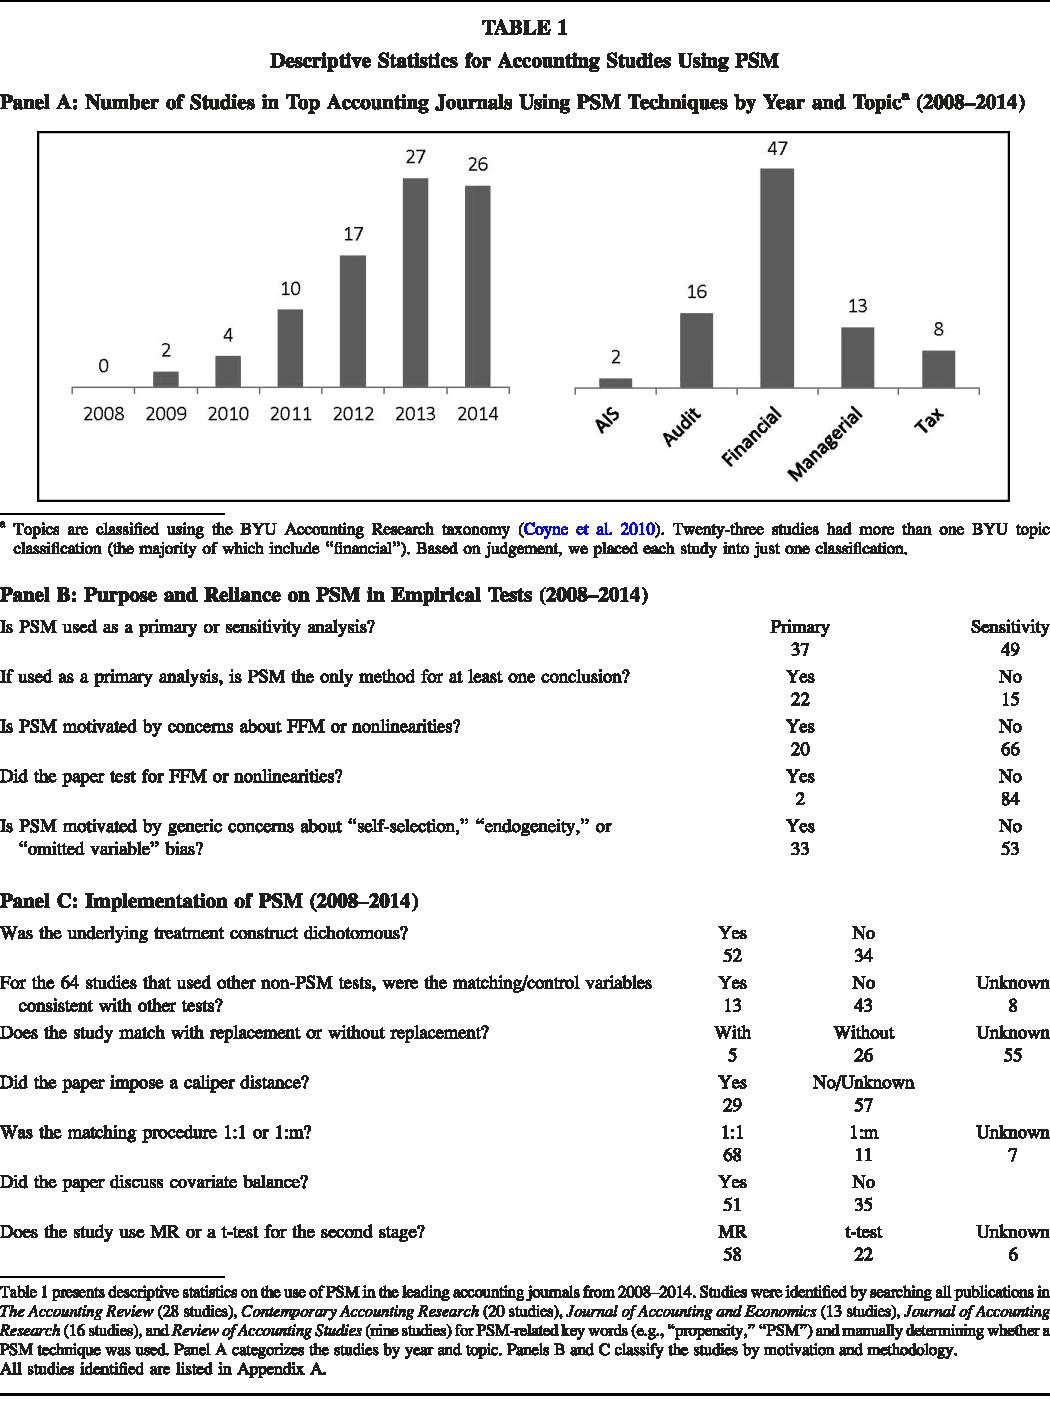
\includegraphics[width=16cm]{../table/tbl01.pdf}
\end{table}

\begin{itemize}
 \item 2008 $\sim$ 2014 年における、\textit{The Accounting Review,
       Contemporary Accounting Research, Journal of Accounting and
       Economics, Journal of Accounting Research, and Review of
       Accounting Studies} に掲載された論文延べ 86 件が対象。
 \item 会計研究で PSM が用いられはじめたのは最近 (86 件中 70 件は 2012
       $\sim$ 2014 の期間に刊行)。
\end{itemize}

\paragraph{各研究の PSM の位置付け (Table 1 Panel B)}

\begin{itemize}
 \item 主要な分析 (primary analyses) として用いている研究が 37 件である
       のに対し、ロバスト・チェック (sensitivity or robustness tests) と
       して用いている研究は 49 件。
 \item PSM を採用する理由として FFM や重回帰分析の線形性の仮定を挙げてい
       る研究はわずか 20 件。
 \item PSM が対処しうる内生性の問題を提示することなく、広く ``自己選択
       (self--selection),'' ``内生性 (endogeneity),'' および ``欠落変数
       バイアス (omitted variable bias)'' への対応として PSM を用いてい
       る研究が 33 件ある。
 \item Heckman (1979) の代わりとして誤用してしまっている研究も存在する。
\end{itemize}

\paragraph{処置群の選択の方法 (Table 1 Panel C)}

\begin{itemize}
 \item 問題の所在
       \begin{itemize}
        \item 処置が 2 値変数 (dichotomous) であるならば、PSM の実施は単純である。
        \item しかしながら、多様な状況でマッチングを実施するため、連続 (あるい
              は順序) 変数に閾値を設けて変換することがある\footnote{2 値
              変数を用いた処置群の選択について、例えば修正再表示のアナウ
              ンスメントや IFRS のアドプションがあげられる。一方で、非 2
              値変数を用いた処置群の選択について、企業の所有構造や監査人
              の産業特殊性 (auditor industry specialization) があげられ
              る}。
       \end{itemize}
 \item 問題点
       \begin{itemize}
        \item このような場合、閾値の近傍の観測値が over--represent される
              傾向があり、それによって、効果の大きさ (および平均処置効果)
              が消失し、第 II 種の過誤が生じる可能性が増大する。
       \end{itemize}
 \item 連続変数を用いている研究の数
       \begin{itemize}
        \item 34 件。また、この影響により、効果の大きさのみならずサンプ
              ル・サイズも低下する。
        \item 59 (12) 件の研究において、MR のサンプル・サイズの大きさは
              PSM の 3 (10) 倍である。
        \item サンプルサイズが小さいほど、サブサンプルは母集団を代表しな
              くなる。
       \end{itemize}
\end{itemize}

\paragraph{コントロール変数の選択 (Table 1 Panel C)}

\begin{itemize}
 \item MR と PSM のいずれを用いるにせよ、同様のコントロール変数を用いる
       べきであるにもかかわらず、しばしば異なるコントロール変数が用いら
       れていることがわかった。
 \item MR からマッチングに用いた変数を除外することは、その変数が処置変数
       (treatment) にも結果変数 (outcome) にも影響を与えないこと、
       ひいては、その変数によるマッチングが不必要であることを意味するに
       他ならない。
 \item 分析においては、\textit{post hoc} なモデルの特定 (model
       specification) をおこなっているという疑念 (appearance; 外観) を避
       けるため、PSM と他のテストとの説明変数の不一致を検討すべきである。
\end{itemize}

\paragraph{傾向スコア推定後のマッチング・プロシージャ (Table 1 Panel C)}

\begin{itemize}
 \item 置換処理 (replace)
       \begin{itemize}
        \item 55 件の研究において、マッチングに際して置換処理がおこなわ
              れているか否か (matching is performed with or without
              replacement) 開示されていない。
        \item 開示している 31 件の研究のうち、5 件が置換あり、26 件が置
              換なしであった。
       \end{itemize}
 \item キャリパー距離 (caliper distance)
       \begin{itemize}
        \item マッチング・プロシージャとしてキャリパー距離を開示して
              いる研究は 29 件のみ。
        \item 開示されているキャリパー距離の分布は、0.00005 から
              0.23 までで、よく用いられている距離は 0.01 (4 件)、0.03 (6
              件)、および 0.10 (5 件) である。
       \end{itemize}
 \item 1 対 1 と 1 対多のどちらのマッチングを用いるか
       \begin{itemize}
        \item 1 対 1 (one--to--one) が 68 instances であるのに対し、1 対
              多 (one--to--many) が 11 instances である。
       \end{itemize}
\end{itemize}

\paragraph{covariate balance (Table 1 Panel C)}

\begin{itemize}
 \item マッチング変数の数 (number of matching variables)、キャリパー距離
       (caliper distance)、グループ・サイズ (group size) などの要因は、
       PSM によってサンプルに covariate balance が生じる程度に影響する。
 \item しかしながら、covariate balance の決定はマッチング・クオリティ
       についての主観的な判断を要求するため、マッチングが実際に適切な
       (sufficient) balance を達成しているか否か、しばしば不透明である。
 \item サーベイの結果、35 件はマッチされたサンプル (matched sample) の
       covariate balance について議論しておらず、4 件のみ傾向スコ
       アの平均差について議論している。
 \item 研究においては、残存した covariate imbalance の効果を緩和するため
       に、PSM のサブサンプルにおいて MR を使うことができる。
 \item サーベイの結果、58 件は (第 2 段階の) ATE を推定する際に MR を用
       いている、22 件は結果変数の距離を t 検定することによって、処置効
       果を推定している、そして、6 件は推定手法を開示していないというこ
       とが明らかとなった。
\end{itemize}

\paragraph{サーベイの結論}

\begin{itemize}
 \item 本節で指摘した問題点は現在の文献でも改善されていない。
 \item Heckman (1979) モデルについて含意を示した Lennox et al. (2012,
       589) の結論と同様に、われわれは、多数の研究が ``重要な計量経済学
       上の問題点および PSM の利用をとりまく問題点に対する理解
       (appreciation) がほとんど無いままに、'' PSM を実施していると結論
       付ける。 
\end{itemize}
\bibliography{./bib/myrefs}
\end{document}
